\section{Theorie}
\label{sec:Theorie}
\subsection{Wechselwirkung von Gammastrahlung mit Materie}
Die Wechselwirkung von hochenergetischen Photonen aus der Gammastrahlung lässt sich auf 3 zentrale Prozesse reduzieren: den Photoeffekt, den Comptoneffekt und die Paarbildung.
In Abbildung \ref{fig:Wechselwirkung} sind die Prozesse schematisch dargestellt.
\begin{figure}[H]
    \centering
    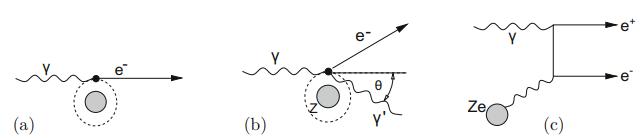
\includegraphics[scale=1.0]{illustration/WWPhoton.png}
    \caption{a) Photoeffekt b) Comptoneffekt c) Paarbildung.\cite{Detektor}}
    \label{fig:Wechselwirkung}
\end{figure}
\noindent Beim Photoeffekt wird das Photon von einem Hüllenelektron vollständig absorbiert und gibt dabei seine gesamte Energie an das Elektron ab. Das Elektron wird dabei aus der Atomhülle gelöst und es entsteht ein freier Platz in der Hülle, 
wenn das Photon genug Energie besitzt, um das Elektron aus der Atomhülle zu lösen. Die Energie des Photons muss dabei mindestens so groß sein wie die Bindungsenergie des Elektrons.
Dies ist bei Photonen der Gammastrahlung der Fall. Dies ist ein Absorptionsprozess. Aufgrund der diskreten Energien der Photonen der Gammastrahlung, der dagegen vernachlässigbaren Bandlücke des Germaniumhalbeiters und 
der Tatsache, dass ein Elektron die volle Energie absorbiert, kann angenommen werden, dass die detektierte Energie dieses Elektron der gesamten 
Energie des Photons entspricht.

\noindent Der Comptoneffekt ist ein Streuprozess, bei dem das Photon an einem freien Elektron gestreut wird. Dabei gibt das Photon einen Teil seiner Energie an das Elektron ab und wird in einem Winkel $\theta$ gestreut.
Das Photon selbst existiert also weiter nach dem Stoß und das Elektron nimmt daher nur einen Teil der Photonenenergie auf. Gemäß der Formel 
\begin{equation}
    \label{eq:Compton}
    E' = \frac{E}{1+\frac{E}{m_0c^2}(1-\cos(\theta))}
\end{equation}
wird die Photonenenergie $E'$ minimal bei Rückstreuung. Daher definiert dieser Punkt die sogenannte Comptonkante, die die maximale Energie der detektierten Elektronen 
definiert, die beim Comptoneffekt beteiligt sind. Der differentielle Wirkungsquerschnitt gibt die Wahrscheinlichkeit an, für eine Streuung in einen bestimmten Raumwinkel.
Für den Comptoneffekt ist dieser Wirkungsquerschnitt gegeben durch die Klein-Nishina-Formel
\begin{equation}
    \label{eq:KleinNishina}
    \frac{d\sigma}{d\Omega} = \frac{r_e^2}{2[1+\epsilon(1-\cos(\theta))]^2}\left(1+cos^2(\theta)+\frac{\epsilon^2(1-\cos(\theta))^2}{1+\epsilon(1-\cos(\theta))}\right)
\end{equation}
mit $\epsilon=\frac{E}{m_0c^2}$ und dem klassischen Elektronenradius $r_e$. In Abbildung \ref{fig:Photo} ist der Wirkungsquerschnitt in Abhängigkeit vom Streuwinkel $\theta$ dargestellt.
In $\phi$-Richtung ist der Wirkungsquerschnitt konstant.
\begin{figure}[H]
    \centering
    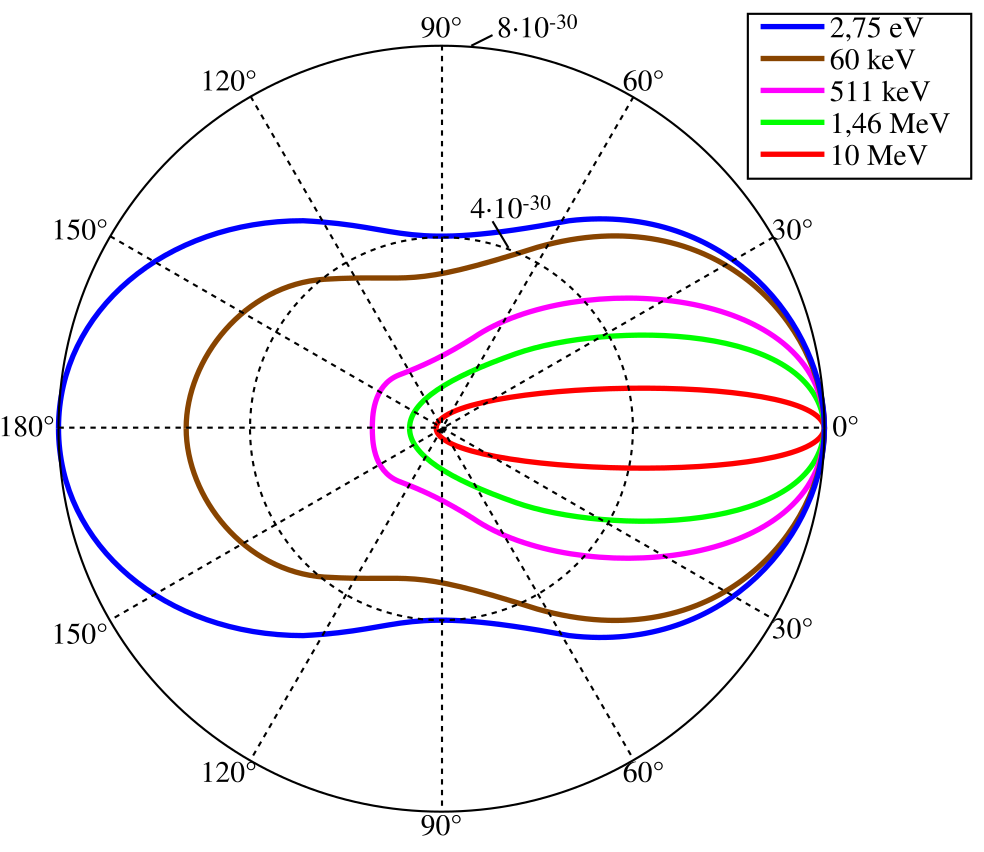
\includegraphics[scale=0.3]{illustration/Klein-Nishina_distribution-en.svg.png}
    \caption{Wirkungsquerschnitt bei Streuung von Photonen an einem Elektron (Compton-Streuung).\cite {Klein}}
    \label{fig:Photo}
\end{figure}

\noindent Die Paarbildung ist ein Prozess, bei dem das Photon in der Nähe eines Atomkerns in ein Elektron-Positron-Paar umgewandelt wird. Dabei muss die Energie des Photons mindestens doppelt so groß sein wie die Ruhemasse des Elektrons.
zusätzlich kann dieser Prozess nur in der Nähe eines Atomkerns stattfinden, da der Impuls des Photons erhalten bleiben muss. Dieser Prozess wird erst bei Photonenenergien deutlich über $1\si{\mega\electronvolt}$ relevant.
Solch hohen Energien werden in diesem Versuch nicht detektiert.

\noindent In Abbildung \ref{fig:Extinktion} ist der Extinktionskoeffizient $\epsilon$ von Germanium in Abhängigkeit von der Energie der Gammastrahlung und der Art der Wechselwirkung dargestellt.
Er gibt an wie stark die Intensität der Gammastrahlung pro Wegstrecke mit $ I(z)=I_0\exp(-\epsilon z)$ abnimmt.
\begin{figure}[H]
    \centering
    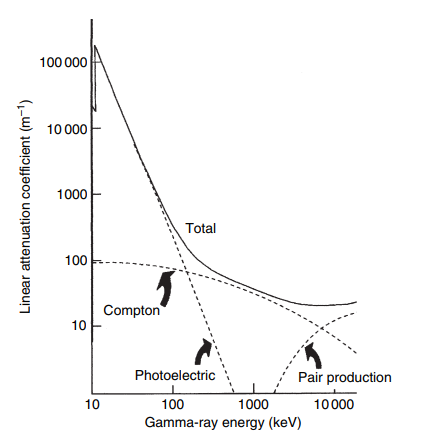
\includegraphics[scale=1.0]{illustration/Extinktionskoeffizient.png}
    \caption{Extinktionskoeffizient von Germanium in Abhängigkeit von der Energie der Gammastrahlung und der Art der Wechselwirkung.\cite{AnleitungAlt}}
    \label{fig:Extinktion}
\end{figure}
\noindent Bei Energien zwischen $100\si{\kilo\electronvolt}$ und $2\si{\mega\electronvolt}$ dominiert der Comptoneffekt, wobei auch der Photoeffekt noch als Vollenergienachweis genutzt werden kann.
Die Interaktionswahrscheinlichkeit steigt beim Comptoneffekt linear mit der Kernladungszahl $Z$ des Absorbermaterials an, während sie beim Photoeffekt quadratisch mit $Z$ ansteigt.
Germanium hat eine relativ hohe Kernladungszahl von $Z=32$, weshalb auch noch viele Photonen über den Photoeffekt detektiert werden können, welcher auf Grund der diskreten 
Energie der Elektronen das Spektrum der Probe am besten charakterisiert. 
\subsection{Gammaspektren}
Ein radioaktives Isotop kann beim Zerfall in andere Isotope in einen angeregten Zustand übergehen. Diesen kann der Atomkern durch spontane Emission eines 
hochenergetischen Photons verlassen. Da ein reines Isotop nur eine endliche Anzahl an Zerfallsmoden besitzt, ist das Spektrum dieser hochenergetischen 
Gammaphotonen charakteristisch für das jeweilige Isotop. In einem Detektor kann dann die Energie der Photonen gemessen werden und ein Spektrum aufgenommen werden.
In ein Abbildung \ref{fig:Spektrum} ist ein Beispiel eines solchen Spektrums dargestellt. Die charakteristischen Linien sind dabei die Vollenergiepeaks die 
entstehen, wenn die Photonen ihre Energie durch den Photoeffekt vollständig im Detektor deponieren. Die Ereignisse abseits der Peaks können 
auf Streuereignisse der Photonen an den Elektronen zurückgeführt werden.
\begin{figure}[H]
    \centering
    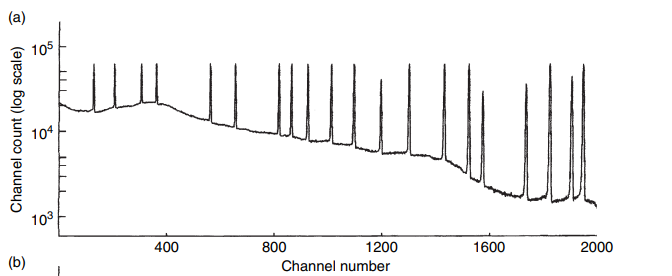
\includegraphics[scale=1.0]{illustration/LinienSpektrum.png}
    \caption{Beispiel eines Gammaspektrums mit charakteristischen Linien.\cite{GammaRay}}
    \label{fig:Spektrum}
\end{figure}
In Abbildung \ref{fig:Mono} ist ein monochromatisches Spektrum dargestellt. Bei Isotopen, die nur in einen angeregten Zustand übergehen können,
werden nur Photonen mit einer Energie detektiert. Dadurch lässt sich am gemessenen Spektrum gut erkennen über welche Prozesse die Strahlung Energie
an den Detektor abgegeben hat. Der Full-Energy-Peak ist dabei der Peak, der durch den Photoeffekt entsteht. Die Comptonkante beschreibt 
den maximalen Energieübertrag auf das Elektron bei Rückstreuung des Photons. Im Comptonkontinuum gibt es einen Backscatterpeak. Dieser entsteht 
durch Rückstreuung von Photonen am Gehäuse des Detektors, welche dann ihre Energie vollständig per Photoeffekt im Detektor deponieren.
Pile-Up beschreibt den Fall, dass zwei Photonen gleichzeitig detektiert werden und als ein Ereignis aufgenommen werden. Die gemeinsame Energie der beiden Photonen sorgt dann für weitere Ereignisse 
jenseits des Full-Energy-Peaks.
\begin{figure}{H}
    \centering
    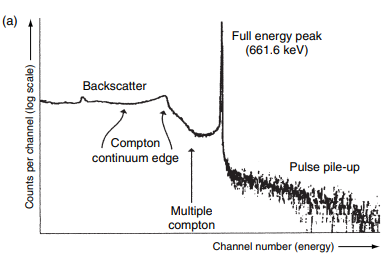
\includegraphics[scale=1.0]{illustration/MonoSpektrum.png}
    \caption{Monochromatisches Gamma-Spektrum.\cite{GammaRay}}
    \label{fig:Mono}
\end{figure}
\noindent Detektiert wird die Anzahl von Ereignissen mit einer bestimmten Energie in einem festen Zeitintervall. Zählexperimente wie dieses
bei denen die Detektionswahrscheinlichkeit konstant bleibt während der Dauer sind immer Poissonverteilt.
Das heißt der Fehler der gezählten Ereignisse ist $\sqrt{N}$, wobei $N$ die Anzahl der Ereignisse ist. 
Bei bekanntem Extinctionskoeffizient kann über die Formel 
\begin{equation}
    \label{eq:Extinktion}
    W=P(d) = 1-\exp(-\epsilon d)
\end{equation}
die Wahrscheinlichkeit berechnet werden, dass ein Photon in einem Detektor mit Dicke $d$ detektiert wird.
Gleichzeitig kann experimentell ein Maß für die Vollenergienachweiswahrscheinlichkeit $Q$ bestimmt werden. Diese gibt an wie wahrscheinlich es ist, dass ein Photon, 
welches von einem bekannten Isotop in Richtung des Detektors emittiert wird und über den Photoeffekt ein Signal erzeugt, detektiert wird.
Es kann über die Formel 
\begin{equation}
    \label{eq:Q}
    Q = \frac{N_{\text{Peak}}}{A\cdot W\cdot t}\cdot\frac{4\pi}{\Omega}
\end{equation}
bestimmt werden. Dabei ist $N_{\text{Peak}}$ die Anzahl der Ereignisse im Peak, $A$ die Aktivität der Probe, $t$ die Messzeit, $\Omega$ der Raumwinkel und $W$ die Emissionswahrscheinlichkeit eines Photons mit dieser Energie.
Der Raumwinkel $\Omega$ ist in diesem experimentellen Aufbau durch den Radius des Detektors und den Abstand zur Probe gegeben.
\begin{figure}[H]
    \centering
    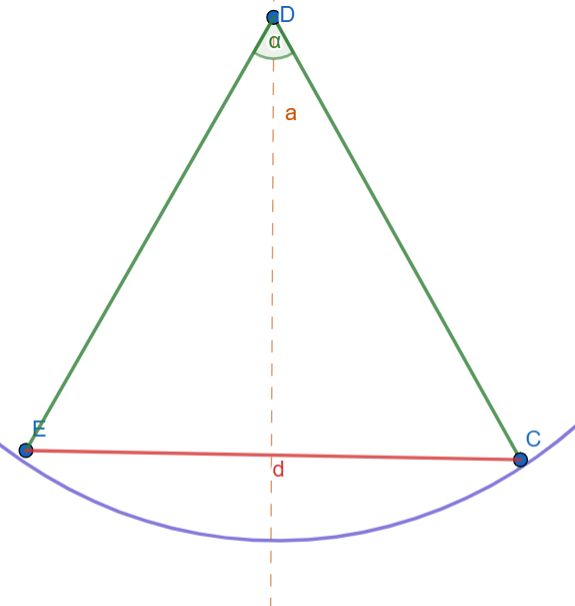
\includegraphics[scale=0.6]{illustration/Raumwinkel.png}
    \caption{Skizze des Versuchsaufbaus.}
    \label{fig:Raumwinkel}
\end{figure}
\noindent Der Raumwinkel ist gemäß den Größen aus Abbildung \ref{fig:Raumwinkel} und der Annahme das $\alpha$ klein ist gegeben durch
\begin{equation}
    \label{eq:Raumwinkel}
    \Omega = 2\pi\left(1-\frac{a}{\sqrt{a^2+r^2}}\right)
\end{equation}
mit $r=d/2$ als Radius des Detektors und $a$ als Abstand zur Probe. Der Abstand $a$ beträgt dabei $7.02\si{\centi\meter}$ von Probe zu einer Aluminiumabschirmung
und $1.5\si{\centi\meter}$ von der Abschirmung zum Detektor. Der Detektor hat einen Radius von $r=2.25\si{\centi\meter}$.
Damit ergibt sich ein Raumwinkel von $\Omega/4\pi=0.016$.
\subsection{Halbleitergrundlagen und Aufbau des Germaniumdetektors}

In Festkörpern mit einem periodischen Gitter kann die Besetzung der Elektronen über eine Bandstruktur beschrieben werden.
Nach dem Pauli-Prinzip können zwei Elektronen in einem System nicht die gleichen Energieniveaus besetzen. Daher spalten sich 
die Energieniveaus der einzelnen Atome in ein Band auf. Genauer sind die Energiebänder die Überlagerungen der Energieniveaus aller Atome im 
reziproken Raum. Dementsprechend können Elektronen mit einer bestimmten Energie im Festkörper nur vorliegen, wenn es Zustände in einem Band mit dieser 
Energie gibt. Energieintervalle ohne Zustand werden Bandlücken genannt, da dort keine Elektronen existieren können.

\noindent Festkörper können anhand ihrer Bandstruktur in 3 Kategorien unterteilt werden: Metalle, Halbleiter und Isolatoren.
Die Bandstruktur dieser Festkörper ist in Abbildung \ref{fig:Band} dargestellt.
\begin{figure}[H]
    \centering
    \includegraphics[scale=0.8]{illustration/Bänder.png}
    \caption{Bandstruktur von Metallen, Halbleitern und Isolatoren \cite{demtröder}.}
    \label{fig:Band}
\end{figure}
\noindent Dabei bezeichnet $E_\text{F}$ die Fermi-Energie, welche angibt bis zu welcher Energie bei $T=\qty{0}{\kelvin}$ die Zustände besetzt sind.
Bei Isolatoren liegt diese Energie zwischen 2 Bändern, also in einer Bandlücke. Das Band unterhalb der Fermi-Energie wird Valenzband genannt, 
da dieses bei $T=\qty{0}{\kelvin}$ vollständig besetzt ist. Das Band oberhalb der Fermi-Energie wird Leitungsband genannt, da dieses bei $T=\qty{0}{\kelvin}$ leer ist und 
Elektronen in diesem Band frei beweglich sind. Bei Metallen liegt die Fermi-Energie im Leitungsband, weshalb diese bei $T=\qty{0}{\kelvin}$ leitfähig sind.
Halbleiter haben eine analoge Bandstruktur zu Isolatoren, jedoch ist die Bandlücke kleiner. Sie beträgt bei Halbleitern bis zu $\qty{3}{\eV}$, bei Isolatoren 
ist sie größer. Daher können in Halbleitern durch thermische Anregung, bei Raumtemperatur etwa $\qty{26}{\milli\eV}$, Elektronen in das Leitungsband gelangen. 
Allerdings ist die Ladungsträgerdichte in Eigenleitung noch sehr gering. Germanium hat allerdings mit einer Bandlücke von $\qty{0.67}{\eV}$ eine relativ geringe Bandlücke, was auch thermische Übergänge 
begünstigt.

\noindent Für eine Erhöhung der Ladungsträgerdichte im Halbleiter kann dieser dotiert werden. Dabei werden gezielt Fremdatome in das Kristallgitter eingebaut, welche zusätzliche Elektronen oder Löcher in das Leitungs- oder Valenzband einbringen.
Diese Fremdatome können in Donatoren und Akzeptoren eingeteilt werden. Ein Donator hat ein Valenzelektron mehr als die Gitteratome des Festkörpers, während die Akzeptoren ein Valenzelektron weniger haben.
Wenn diese nur in geringer Anzahl eingebaut werden, verändern sie die Bandstruktur des Festkörpers nahezu nicht. Sie können allerdings Zustände innerhalb der Bandlücke 
erzeugen und so die Bandlücke stark verkleinern. In Abbildung \ref{fig:Ndot} ist 
die Bandstruktur eines N-dotierten Halbleiters dargestellt. Dort ist zu sehen, dass die Energieniveaus der Donatoren deutlich näher am Leitungsband liegen. 
Dadurch ist die Bandlücke sehr klein und die Ladungsträger können bei Raumtemperatur nahezu alle ins Leitungsband gelangen.
\begin{figure}[H]
    \centering
    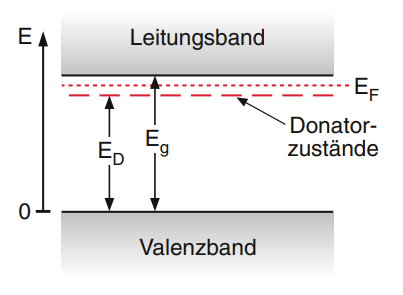
\includegraphics[scale=0.8]{illustration/Ndot.png}
    \caption{Bandstruktur eines N-dotierten Halbleiters \cite{demtröder}.}
    \label{fig:Ndot}
\end{figure}
\noindent Der Germaniumdetektor wird nicht dotiert, sondern  mit Lithium und Gold beschichtet. Diese wirken wie eine n oder p dotierte Schicht in dem Sinne, dass Lithium 
Elektronen in das Leitungsband einbringt und Gold Löcher in das Valenzband. Dadurch entsteht eine Verarmungsschicht im Germaniumkristall, in der die Ladungsträgerdichte sehr gering ist. 
Germanium selbst ist ein indirekter Halbleiter, siehe Abbildung \ref{fig:Indirekt}, was bedeutet, dass die Bandkante des Leitungsbandes nicht am gleichen Punkt im reziproken Raum liegt wie die Bandkante des Valenzbandes.
Für Übergänge zwischen den beiden Bändern bedeutet dies, dass ein Phonon benötigt wird, um den Impulsunterschied auszugleichen. Dies macht den Prozess unwahrscheinlicher und es werden größere
Energien benötigt um die Bandlücke zu überwinden. 
\begin{figure}[H]
    \centering
    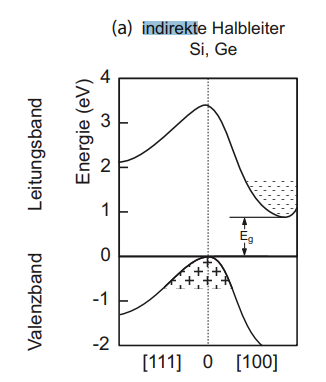
\includegraphics[scale=1.0]{illustration/Indirekter Halbleiter.png}
    \caption{Bandstruktur eines indirekten Halbleiters \cite{Detektor}.}
    \label{fig:Indirekt}
\end{figure}
\noindent Um den dotierten Germaniumkristall als Detektor zu verwenden wird nun eine Spannung so angelegt, dass die Ladungen und Löcher in den dotierten Schichten abfließen.
Im Kristall selbst diffundieren alle Elektronen zu der p-dotierten Schicht und alle Löcher zu der n-dotierten Schicht. Die zusätzlich angelegte 
Spannung verstärkt diesen Effekt noch. Die Verarmungsschicht umfasst dann den gesamten Kristall. Zwischen den dotierten Schichten entsteht ein elektrisches Feld, welches
entstehende freie Ladungsträger sofort absaugt. Wenn nun ein hochenergetisches Photon ein Elektron aus dem Valenzband in das Leitungsband 
anhebt. Entsteht ein Elektron-Loch-Paar. Das Elektron selbst ist wieder hochenergetisch und löst so weitere Elektronen-Loch-Paare aus.
Auf Grund des E-Feldes sammeln sich die Elektronen und Löcher jeweils an einem Pol, wo sie detektiert werden können. Die Anzahl an Ladungen ist dann ungefähr proportional zur Energie des Photons.
\subsection{Signalverarbeitung und Unsicherheiten}
Die Elektronik hat im Prinzip 3 verschiedene Aufgaben. Zunächst muss die Ladungsmenge, die ein Photon erzeugt hat in ein elektrisches Signal umgewandelt werden, z.B. einen Spannungspuls.
Diese Aufgabe übernimmt der Vorverstärker. Dann soll das Signal so verstärkt und geformt werden, dass sich die verschiedenen Signale gut unterscheiden lassen. Das macht der Verstärker 
zusammen mit einem Shaper und einem Diskriminator. Zuletzt soll das Signal gemäß seiner Stärke digitalisiert und gespeichert werden. Dies übernimmt ein Multichannelanalyzer (MCA).
Einen schematischen Aufbau der Elektronik ist in Abbildung \ref{fig:Schaltung} dargestellt.
\begin{figure}
    \centering
    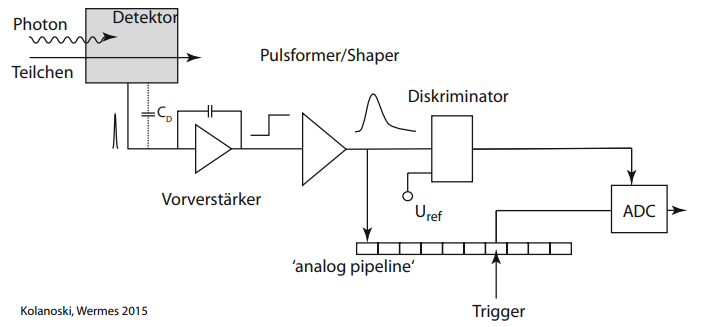
\includegraphics[scale=0.8]{illustration/Messchaltung.png}
    \caption{Vollständige Messschaltung eines Germaniumdetektors\cite{Detektor}.}
    \label{fig:Schaltung}
\end{figure}
\noindent In der Vorverstärkerstufe wird das Signal mit einem über einen Kondensator rückgekoppelten Operationsverstärker integriert, sodass ein Spannungssignal proportional zur Ladungsmenge entsteht.
Parallel zum Kondensator ist ein großer Widerstand für die Entladung des Kondensators, geschaltet. Die Integriererschaltung zusammen mit dem resultierenden Signal ist in Abbildung \ref{fig:PreAmp} dargestellt.
\begin{figure}[H]
    \centering
    \includegraphics[scale=0.8]{illustration/Vorverstärker.png}
    \caption{Vorverstärker in einem Germaniumdetektor \cite{Detektor}.}
    \label{fig:PreAmp}
\end{figure}
\noindent Die Folgende Elektronik soll das Signal so Formen, dass jeder Puls eine Gaußform annimmt. Wenn die Signale eine einheitliche Form haben, kann mit einem Diskriminator
Pulse mit geringer Spannung herausfiltern. So können Rauscheinflüsse in dem resultierenden Spektrum minimiert werden. 
Der Multichannelanalyzer sortiert die Signale dann nach ihrer Stärke und speichert sie gemäß ihrer Stärke in einem Kanal ein. Dieser Prozess führt ein Analog-Digital-Wandler durch.
Der kontinuierlichen Signalstärke wird eine diskrete Zahl zugeordnet. 
Die Kanäle können dann mit einem Computer ausgelesen werden.

\noindent Das Gammaspektrum kann niemals vollständig scharf aufgelöst werden. Das hat sowohl physikalische Ursachen als auch technische.
Ein wesentlicher Beitrag entsteht durch das Rauschen in der Elektronik des Detektors. Dieses Rauschen, bedingt durch die Verstärkerschaltung und andere elektronische Komponenten, 
führt zu einer Schwankung im Signal und damit zu einer Verbreiterung der spektralen Linien.
Weiterhin spielen thermische Übergänge zwischen den Bändern des Germaniumkristalls eine Rolle. Diese sorgen für ein kontinuierliches Signal, welches sich mit echten 
Signalen überlagert.
Eine gute Kühlung des Germaniumdetektors hilft, 
diese thermischen Effekte zu minimieren, aber sie können nicht vollständig unterdrückt werden.
Auch die Schwankungen in der Anzahl der erzeugten und detektierten Elektronen tragen zur Linienbreite bei. 
Bei jedem einfallenden Gammaquant wird eine gewisse Anzahl von Elektron-Loch-Paaren erzeugt, die jedoch statistischen Schwankungen unterliegen, was zur weiteren Verbreiterung der Spektrallinien führt.
Das Abschirmmaterial reduziert Hintergrundstrahlung und Streustrahlung, die das Spektrum verzerren könnten. Für den Versuchsaufbau musste die Abschirmung allerdings etwas offen gelassen werden.



% \begin{equation}
%     \label{eq:}

% \end{equation}
% \begin{figure}[H]
%     \centering
%     \includegraphics[scale=0.5]{content/}
%     \caption{\cite{}.}
%     \label{fig:}
% \end{figure}

%\cite{}
